\section{Konsekvens}
Ved implementering af Event sourcing opnås et system der kan reagere på hændelser, som dette lytter på. Dette kan sørge for, at ved at lytte på disse events kan opnå den ønskede funktionalitet, når f.eks en skriving til en database er foretaget.

Det kan om Event sourcing tilføjes, at disse events bliver rejst når en begivenhed indtræffer, men at dette ikke nødvendigvis betyder, at der ikke samme tid er en ny event på vej. Dette kan lede til inkonsistent data, hvor der læses noget data der kan være ændret siden eventet der reageres på er indtruffet.

Dertil kan det være, at Event Store'en indeholder så mange events, at et sytem kan tage lang tid at initiere, da mange handlinger kan være foretaget. Dette kan dog løses ved at inddrage \textbf{Snapshots}, som sørger for, at sætte et state, hvor alle de nødvændige ting er til rådighed. Derefter kan de efterfølgende events udføres og dataen opsummeres.

Ved implementering af Event sourcing stiger kompleksiteten af systemet, som tidligere nævn, hvilket betyder at Event sourcing ikke altid er fortrukket. 

Herunder er der listet nogle eksempler på systemer, hvor Eventsourcing bør overvejes.
\begin{itemize}
	\item Applikationer, hvor der kan drages direkte paralleer til den event drevne virkelighed
	\item Applikationer, hvor det er en nødvendighed, at det ikke opstår konflikt ved dataopdatering 
	\item Applikationer, hvor en opdatering, ved ny tilgængeligt data, er en nødvendighed
	\item Applikationer, hvor muligheden for at ramme et forgående stadie er en nødvendighed.
	\item Applikationer, hvor kompleksiteten i systemet og domænet i forvejen er høj.
\end{itemize}

Event sourcing er ofte brugt brugt sammen med \textbf{CQRS}, da dette kan medvirke til at dette pattern bliver mere indbringende, da skrive- og læseoperationerne bliver koblet i en Event store og derfor kan sørge for at disse har kendskab til hinandens stadier.

\begin{figure}[H]
	\center
	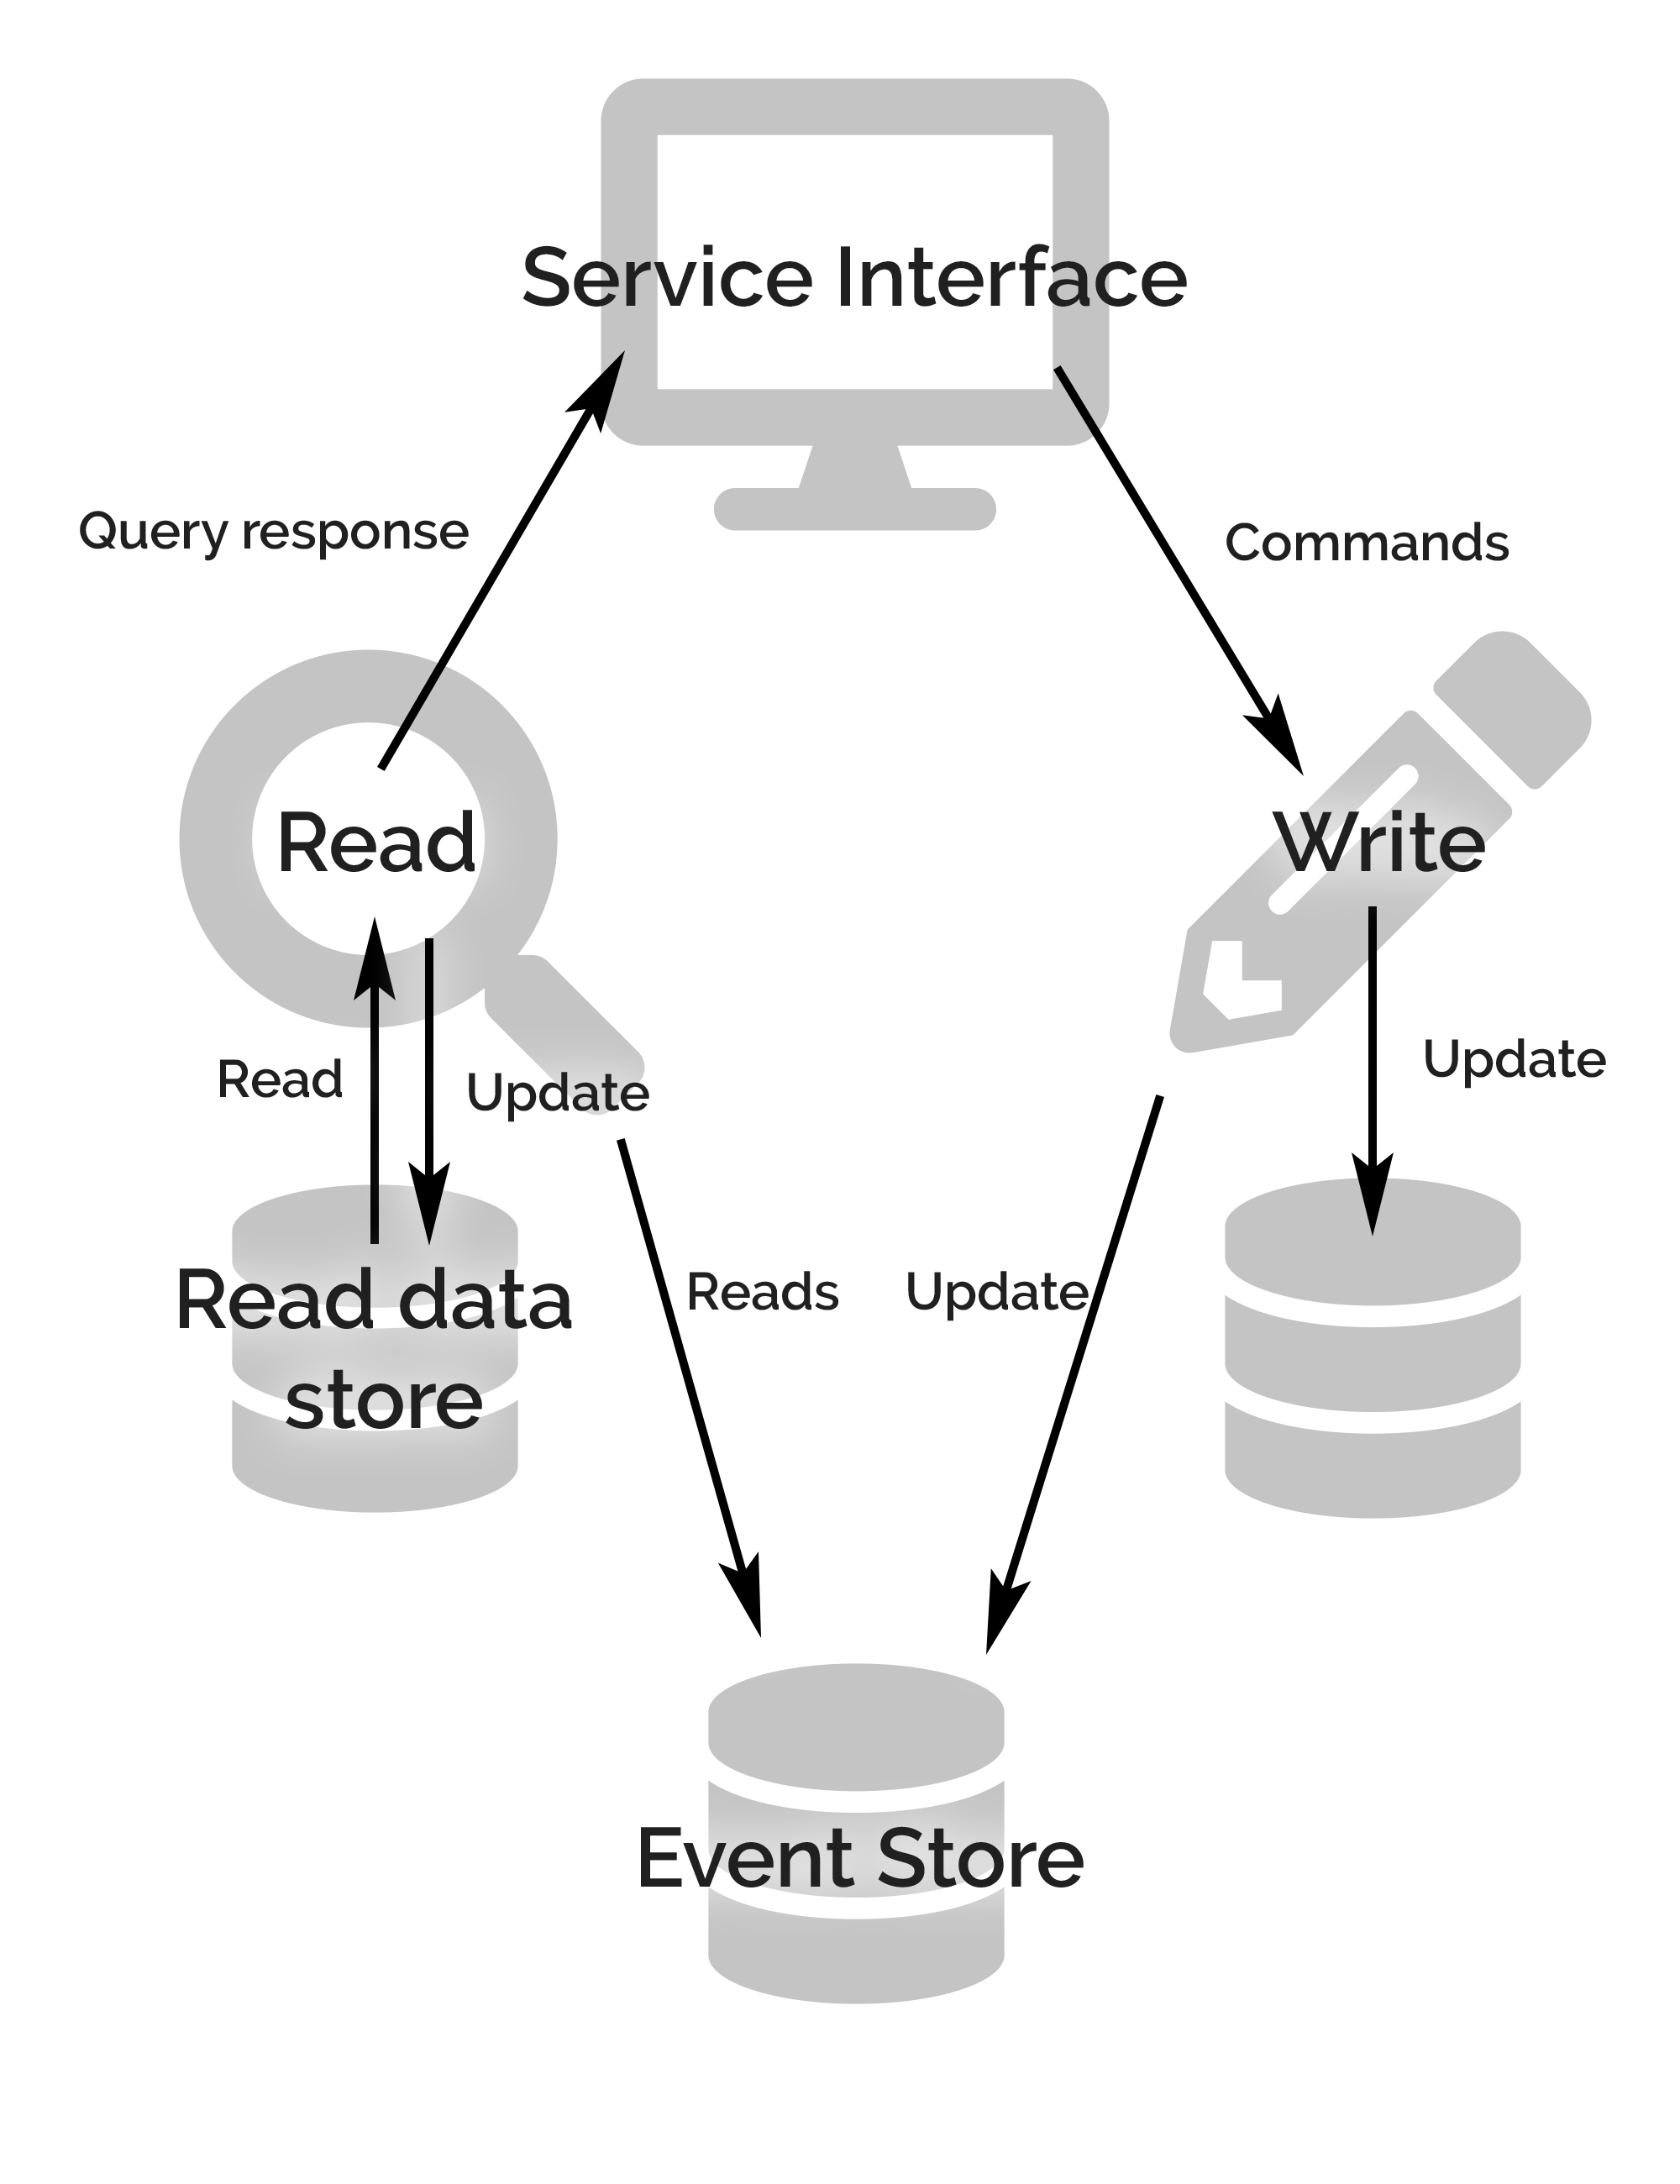
\includegraphics[width=0.5\textwidth]{ES-Model.png}
	\caption{Simpel CQRS med Read og Write}
	\label{fig:cqrs-ES_model}
\end{figure}
\fxnote{Ændre til nyt billede hvor ES er tilføjet og ændre billedtekst}

På ovenstående figur \ref{fig:cqrs-ES_model} er det vist, hvor Event sourcing tilføjes til \textbf{CQRS}-pattern'et og hvordan dennes effekt indtræffer. her ses det at skrivesiden kan opdatere Event Store og dermed notificere læsesiden, som nu ved at der er ny data tilgængelig, og kan nu foretage en ny iteration af Event Store'ens Events.